\newpage
\section{Iteración 2: Prototipo mejorado}

\subsection{Introducción}
En el marco de la iteración anterior, se desarrolló un prototipo funcional que permitió validar la viabilidad técnica del sistema propuesto y sentar las bases para su evolución. Este trabajo destacó por identificar áreas clave de mejora que podrían optimizar su desempeño. Con base en estos hallazgos, la presente iteración se enfoca en mejorar el prototipo inicial, explorando la implementación de compensaciones en el sistema de control. Este enfoque tiene como objetivo principal incrementar la precisión, robustez y eficiencia del sistema, marcando un hito significativo en su desarrollo.

\subsection{Requerimientos}
En esta iteración abordaremos los siguientes requerimientos funcionales:

\begin{center} \begin{tabular}{|c|c|}
\hline
    ID & Descripción \\
\hline
    RF4 & El robot debe poder realizar trayectorias en línea recta y curvas. \\ 
\hline
    RF5 & El robot debe poder corregir su trayectoria mediante el uso de sensores. \\ 
\hline
\end{tabular} \end{center}

Por otra parte, los requerimientos no funcionales que trataremos son:

\begin{center} \begin{tabular}{|p{0.10\linewidth}|p{0.65\linewidth}|}
\hline
    ID & Descripción \\
\hline
    RNF1 & Debería tener tiempos de respuesta aceptables para el buen funcionamiento del sistema de control. \\
\hline
    RNF2 & El software debería contar con pruebas unitarias y de integración. \\
\hline
    RNF4 & El código debería contar con documentación.\\
\hline
\end{tabular} \end{center}

\subsection{Desarrollo}

\subsubsection{Compensación del modelo cinemático}

Dado el potencial del modelo cinemático, procedimos a compensar el sistema mediante la información provista por éste.

\paragraph{Compensación de movimiento lineal} \mbox{} \vspace{8pt}

En un caso real, existen variaciones que pueden provocar desviaciones en la ruta planeada debido a la textura o inclinación del suelo, imprecisiones o ruido en los sensores y el desgaste de las ruedas, así como otros factores mecánicos que pueden alterar la respuesta del robot a las órdenes de control.

Para abordar estos desafíos, se implementa un procedimiento de control que ajusta continuamente las velocidades de las ruedas en función de la retroalimentación recibida de los sensores y del modelo cinemático del robot. Se utilizan sensores para medir la posición y orientación actual del robot en el plano, inferida a partir de la odometría y las velocidades de las ruedas, para comparar estos datos con la trayectoria deseada y estimar los errores de posición y orientación. El modelo cinemático nos ayuda a  comprender cómo las velocidades de las ruedas individuales afectan el movimiento general del robot a través de ecuaciones matriciales que describen el comportamiento cinemático del robot.

Basado en los errores estimados y el modelo cinemático, se calculan las correcciones necesarias para las velocidades de las ruedas y se envían a los actuadores de las ruedas, logrando que el robot ajuste su movimiento de manera inmediata. \cite{rijalusalamkinematics} El proceso de medición, estimación, cálculo y aplicación de correcciones se repite continuamente a una frecuencia de $500[ms]$, equivalentes a 5 períodos de medición de RPM de cada rueda. En la Figura \ref{fig:diagramamodelocinemcompensado} podemos ver como se relacionan las variables.

\begin{figure}[htb]
    \centering
    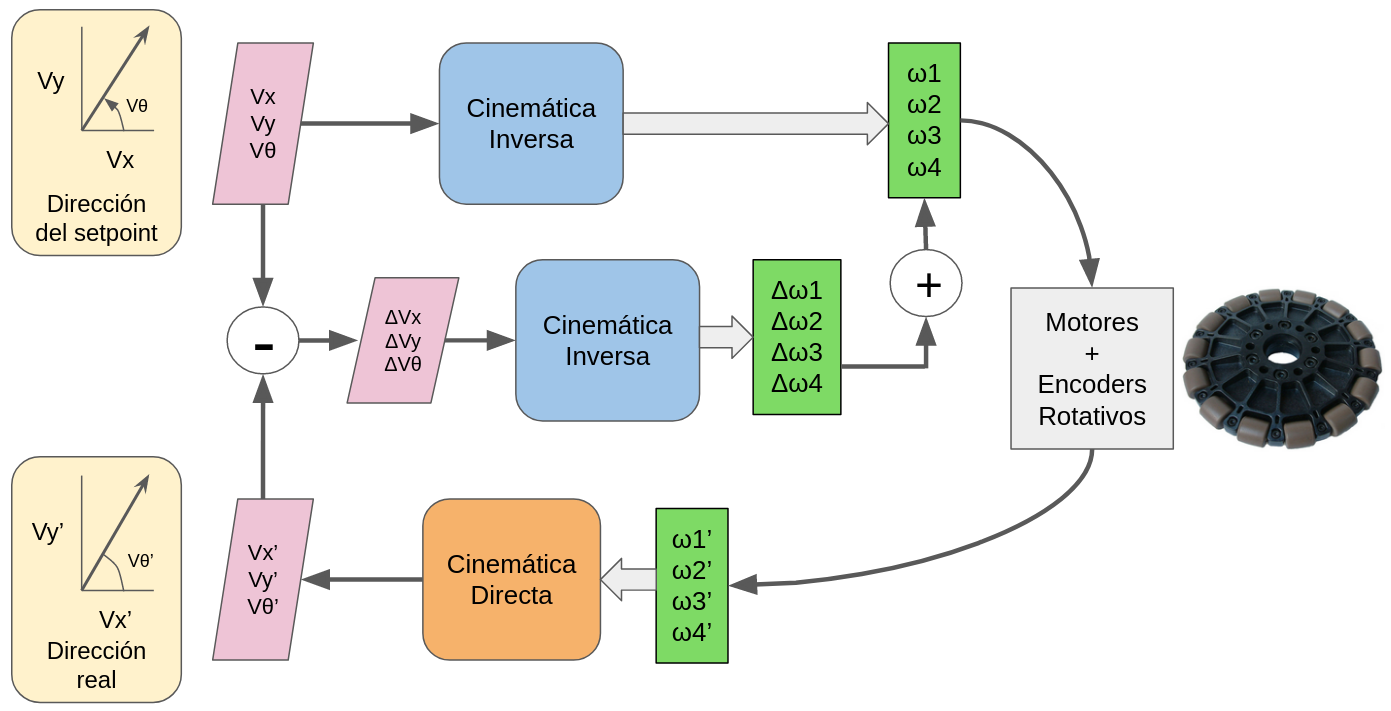
\includegraphics[width=1\linewidth]{images/diag_compensacion_modelo_cinem.png}
    \caption{Diagrama del Modelo Cinemático compensado}
    \label{fig:diagramamodelocinemcompensado}
\end{figure}

Los experimentos se realizaron en un entorno consistente con la iteración anterior y los resultados muestran una reducción significativa en los errores de trayectoria, demostrando la robustez del enfoque propuesto, de modo que el robot puede seguir trayectorias con desviaciones mínimas.

\paragraph{Compensación de movimiento rotacional} \mbox{} \vspace{8pt}

El enfoque propuesto es el de tener un acumulador basado en la odometría de $\theta$ que mide la distancia recorrida angularmente. El principio de funcionamiento es tal que aplica ajustes en la velocidad rotacional para compensar el desplazamiento, de modo que el robot intente llevar la distancia rotacional a cero nuevamente. Por ejemplo, si el robot detecta un desplazamiento hacia la derecha, se aumenta la velocidad rotacional hacia la izquierda para compensar el desfase en la cantidad determinada por la distancia rotacional. De este modo es posible corregir la orientación de movimiento. \\

En la Figura \ref{fig:diagsecuenciamodcinemcompens} se muestra un diagrama de secuencia sobre la implementación de la compensación del Modelo Cinemático.

\begin{figure}[htb]
    \centering
    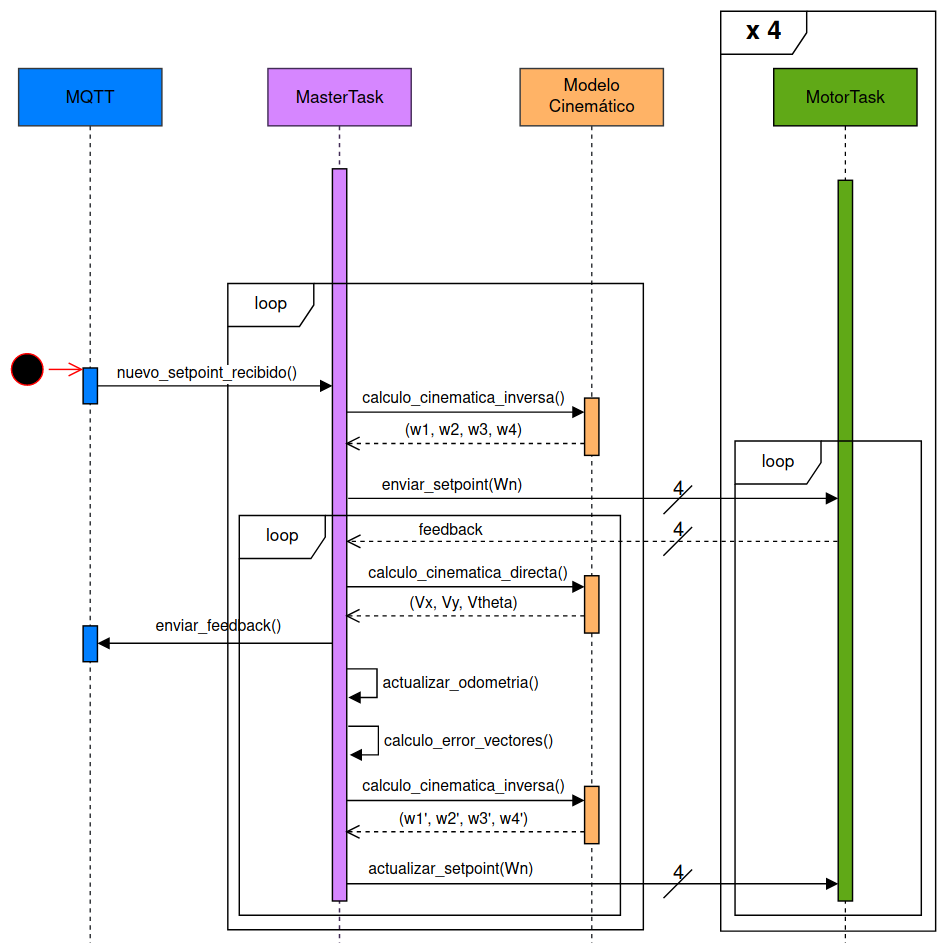
\includegraphics[width=1\linewidth]{images/diag_secuencia_modelo_cinematico_compensado.png}
    \caption{Diagrama de secuencia del Modelo Cinemático compensado}
    \label{fig:diagsecuenciamodcinemcompens}
\end{figure}




\subsubsection{Seguidor de línea}

A pesar de ser una herramienta fundamental para estimar la posición y orientación del robot, la odometría está sujeta a errores. Por lo que se hace necesario contar con un mecanismo adicional para poder detectar desviaciones en la trayectoria. Para esto se propone un seguidor de línea colocado de modo que el robot pueda detectar cuando se sale por fuera de las trayectorias determinadas por las líneas.

Un seguidor de línea es un sistema basado en sensores que detectan marcas en el entorno y utilizan esta información para ajustar la trayectoria del robot de manera automática.

La implementación de un seguidor de línea en robots omnidireccionales ofrece varias ventajas. En primer lugar, permite corregir desviaciones causadas por errores acumulativos en la odometría, ya que los sensores del seguidor de línea proporcionan información directa sobre la posición del robot respecto a la línea de referencia y en tiempo real.


\paragraph{Elección de método de seguimiento} \mbox{} \vspace{6pt}

Existen distintas técnicas para detectar una linea que un robot puede seguir. \\

\textbf{Seguidor de Línea Ultrasónico} \mbox{} \vspace{6pt} \\
Utiliza sensores ultrasónicos para detectar la presencia de una línea guía de la cual el robot debe mantenerse equidistante. Estos sensores emiten ondas sonoras de alta frecuencia y miden el tiempo que estas tardan en reflejarse al encontrar una superficie, lo que permite al robot seguir una trayectoria de manera precisa.

Entre sus ventajas, destaca su robustez, ya que no se ven afectados por factores como la suciedad o la iluminación, y su precisión, al detectar con alta exactitud la distancia hacia la línea guía. Sin embargo, estos sistemas presentan algunas desventajas, como la mayor complejidad y costo asociados con los sensores ultrasónicos, así como un alcance limitado en comparación con otros tipos de sensores. \cite{venkateshrfidultrasonic} \cite{aungultrasonic} \\


\textbf{Seguidor de Línea por Cámara} \mbox{} \vspace{6pt} \\
El seguidor de línea por cámara utiliza cámaras y algoritmos de procesamiento de imágenes para identificar y seguir líneas en el suelo de manera eficiente. Estas tecnologías permiten que el sistema sea altamente versátil, adaptándose a distintos tipos de líneas y patrones, al tiempo que proporcionan información adicional sobre el entorno que rodea al robot.

No obstante, esta solución presenta ciertos desafíos. Por un lado, requiere algoritmos avanzados de procesamiento de imágenes, lo que puede complicar su implementación. Por otro, su desempeño puede verse afectado por cambios en las condiciones de iluminación, lo que limita su eficacia en entornos variables. \cite{inianlinefollowcamera} \\


\textbf{Seguidor de Línea Ópticos} \mbox{} \vspace{6pt} \\
Los seguidores de línea ópticos son una de las implementaciones más comunes, ya que emplean sensores ópticos para detectar el contraste entre una línea dibujada en el suelo, generalmente negra, y el fondo, que suele ser blanco. Sensores como los fotodiodos o fototransistores envían señales al controlador del robot, permitiéndole ajustar su trayectoria para mantenerse sobre la línea. Entre las opciones disponibles, las versiones láser o infrarrojas son las más utilizadas.

Este sistema tiene como principales ventajas su simplicidad y bajo costo, ya que es relativamente sencillo de implementar, así como la amplia disponibilidad de estos dispositivos en el mercado. Sin embargo, también presenta algunas desventajas. Su rendimiento puede verse afectado por factores ambientales como la iluminación variable, el polvo, la suciedad y las superficies reflectantes, además de mostrar menor precisión en superficies no uniformes. Adicionalmente, las líneas pintadas en el suelo pueden desgastarse con el tiempo, requiriendo mantenimiento constante. \\


\textbf{Seguidor de Línea Magnético} \mbox{} \vspace{6pt} \\
El seguidor de línea magnético utiliza bandas magnéticas adheridas al suelo o a una pared, las cuales son detectadas por sensores magnéticos. Estos sensores identifican cambios en el campo magnético, permitiendo al robot seguir con precisión la trayectoria marcada por las bandas magnéticas.

Entre las ventajas de este sistema se encuentra su inmunidad al entorno, ya que no es afectado por factores como la suciedad, el polvo, la iluminación variable o las superficies reflectantes. Además, las bandas magnéticas destacan por su durabilidad, resistiendo condiciones ambientales adversas y requiriendo poco mantenimiento, mientras que ofrecen alta precisión en la navegación, especialmente en entornos industriales. Sin embargo, este sistema también presenta desventajas, como el mayor costo asociado a los sensores y bandas magnéticas en comparación con sistemas ópticos, así como el tiempo y esfuerzo necesarios para instalar dichas bandas. \\


\textbf{Seguidor de Línea con Etiquetas RFID} \mbox{} \vspace{6pt} \\
El seguidor de línea con etiquetas RFID utiliza etiquetas RFID incrustadas en el suelo o las paredes, junto con lectores RFID instalados en el robot, para detectar la presencia y posición de dichas etiquetas. Este sistema permite al robot interpretar su entorno de forma más inteligente al acceder a la información adicional almacenada en las etiquetas.

Entre las ventajas de este enfoque se encuentran la capacidad de las etiquetas RFID para proporcionar información adicional que facilita una navegación más eficiente, su inmunidad a factores ambientales como suciedad, polvo, variaciones en la iluminación o superficies reflectantes, y su flexibilidad para diseñar trayectorias más complejas y adaptativas. Sin embargo, presenta algunas desventajas, como el alto costo asociado a los sistemas RFID debido al precio tanto de los lectores como de las etiquetas, así como la mayor complejidad requerida para su implementación y configuración en comparación con otros sistemas. \cite{venkateshrfidultrasonic} \\


Al evaluar las diferentes alternativas, optamos por un seguidor de línea magnético dado que es el que mejor se adapta a los requerimientos de funcionamiento del robot. Una de las principales ventajas es la inmunidad a las condiciones del entorno y su relativo bajo costo. No se ven afectados por elementos que pueden interferir con los sensores ópticos, como la suciedad, el polvo, la iluminación variable, superficies reflectantes o las sombras. Esta característica aumenta la robustez del sistema en entornos industriales o comerciales donde las condiciones pueden ser menos que ideales.

Otra ventaja importante es la durabilidad y el mantenimiento reducido. Las bandas magnéticas son resistentes al desgaste y pueden soportar condiciones ambientales variables, reduciendo la necesidad de mantenimiento frecuente y aumenta la vida útil del sistema. En comparación, en caso de un sensor óptico, las líneas pintadas o adhesivas pueden desgastarse con el tiempo y requerir repintado o reemplazo periódico. Además, se pueden colocar de manera discreta dado que no es necesario que sean visibles.


\paragraph{Implementación} \mbox{} \vspace{10pt}

Se hizo una pieza impresa en 3D y se colocaron los sensores una determinada distancia entre sí obtenida experimentalmente. El arreglo de sensores Hall se coloca en el frente del robot y se mejoro la pista adhiriendo los imanes.

El procedimiento para compensar el robot se basa en que al tocar un imán de los extremos significa que existe una determinada distancia angular que difiere del vector de dirección deseado. Se representa esta distancia mediante $d_{r\theta}$:

\begin{figure}[H]
    \centering
    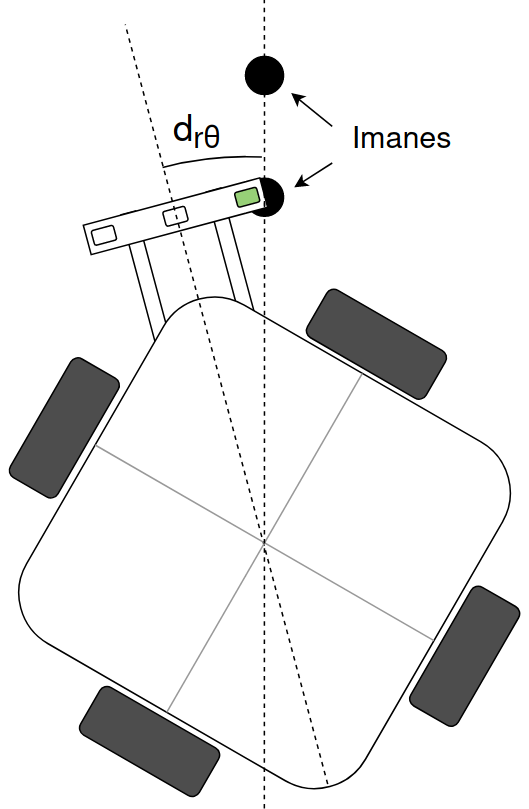
\includegraphics[width=0.4\linewidth]{images/robot_desplazamiento_angular_toca_iman.png}
    \caption{Escenario de detección de un imán}
    \label{fig:deteccionimanrobot}
\end{figure}

El enfoque propuesto es el de tener un acumulador que mide la distancia recorrida angularmente y ajusta la velocidad rotacional para compensar el desfase. Cada vez que se detecta un imán se suma o se resta un determinado valor de distancia angular de modo que el controlador intente llevarla a 0 nuevamente. Por ejemplo, si el robot detecta un desplazamiento hacia la derecha, se aumenta la velocidad rotacional hacia la izquierda.

El algoritmo de control opera de la siguiente manera:

\begin{enumerate}
    \item Los sensores magnéticos son monitoreados continuamente para detectar la presencia de imanes. Cada vez que se detecta un imán en alguno de los extremos, se actualiza un acumulador de distancia angular recorrida sumando o restando un valor determinado. Este valor depende de la distancia de los sensores al centro del robot y de la distancia entre los mismos.

    \item El objetivo es que el acumulador se mantenga en cero, lo que indicaría que el robot sigue la dirección de la trayectoria. El sistema de control ajusta las velocidades de las ruedas del robot en tiempo real en función al desplazamiento angular detectado.    
\end{enumerate}

Al realizar las pruebas, se lanzó al robot en distintas circunstancias, comenzando alineado con los imanes y comenzando con una desviación detectable. A medida que se avanzaron los ensayos se fue iterando sobre los coeficientes del seguidor de línea para compensar el error.

En una primera instancia, la implementación de la corrección del desplazamiento angular estaba dado por una velocidad fija. En las sucesivas experiencias, notamos que el robot a bajas velocidades se comportaba de un modo esperado y que a medida que se incrementaba la velocidad era menos estable. Es por ello que se cambió la velocidad constante por una que sea variable según la velocidad lineal del robot, es decir, ahora la compensación es adaptativa. De modo que a mayor velocidad lineal, mayor velocidad rotacional para realizar la compensación. Esto se debe a la inercia del robot, implicando que a mayor velocidad requiere mayor compensación para vencer el momento del mismo.

En la Figura \ref{fig:diagsecuencialinefollowmodcin} se detalla un diagrama de secuencia del funcionamiento del modelo cinemático compensado con el seguidor de línea.

\begin{figure}[H]
    \centering
    \hspace*{-1.25cm}
    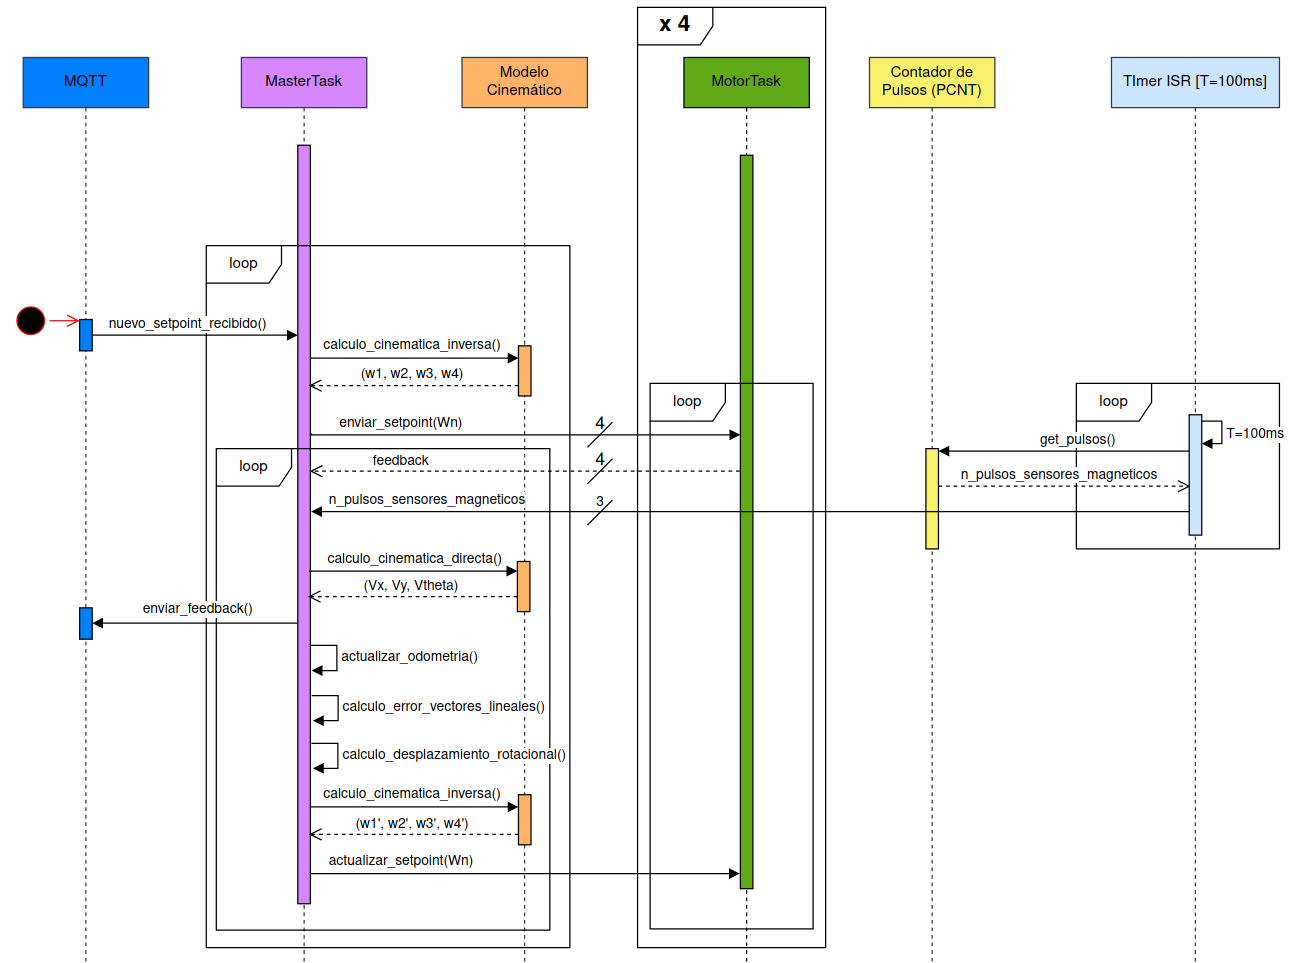
\includegraphics[width=1.2\linewidth]{images/diag_secuencia_seguidor_linea_magnetica_modelo_cinem_compensado.png}
    \caption{Diagrama de secuencia del seguidor de linea con el Modelo Cinemático}
    \label{fig:diagsecuencialinefollowmodcin}
\end{figure}


\subsection{Testing y pruebas}

Las pruebas realizadas en esta iteración parten del prototipo logrado en la iteración anterior.

\begin{testtableformat}
    \hline \rowcolor{test_header_color}
        Test ID             & TC\_02\_00 \\
    \hline
        Tipo de test        & Test de integración \\
    \hline
        Objeto de prueba    & Modelo Cinemático \\
    \hline
        Requerimiento       & RF4 - RF5 \\
    \hline
        Nombre              & Modelo Cinemático con compensación en línea recta \\
    \hline
        Descripción         & Comprobar que el Modelo Cinemático compensa adecuadamente las velocidades de las ruedas según un setpoint en línea recta \\
    \hline
        Precondición        & PRECOND\_B \\
    \hline
        Pasos del test      & \begin{enumerate}
                                \item Enviar al robot un setpoint con distancia entre [50cm $\sim$ 400cm] y velocidad lineal entre $\pm$[0.25m/seg $\sim$ 0.75m/seg]
                                \item Verificar que el robot recorre el vector dado a lo largo de la distancia determinada y que su movimiento es compensado
                                \item Repetir desde el paso 1) con diferentes valores
                            \end{enumerate} \\
    \hline
        Resultado esperado  & El robot se mueve en línea recta en la dirección del vector dado por $V_x$ y $V_y$. Debe ser notable la mejora en la estabilidad del vector a realizar. \\
    \hline
        Resultado obtenido  & Se observa que el robot mejora sustancialmente el desempeño al realizar la trayectoria. \\
    \hline
        Observaciones       & - \\
    \hline
\end{testtableformat}


\begin{testtableformat}
    \hline \rowcolor{test_header_color}
        Test ID             & TC\_02\_01 \\
    \hline
        Tipo de test        & Test de integración \\
    \hline
        Objeto de prueba    & Seguidor de línea magnética - Modelo Cinemático \\
    \hline
        Requerimiento       & RF5 \\
    \hline
        Nombre              & Compensación de linea magnética \\
    \hline
        Descripción         & Verificar que el robot compensa su trayectoria al comenzar centrado en la línea de imanes \\
    \hline
        Precondición        & PRECOND\_C \\
    \hline
        Pasos del test      & \begin{enumerate}
                                \item Colocar al robot centrado respecto a la línea de imanes
                                \item Enviar al robot un setpoint con distancia entre [50cm $\sim$ 400cm] y velocidad lineal entre $\pm$[0.25m/seg $\sim$ 0.75m/seg]
                                \item Verificar que el robot recorre el vector dado a lo largo de la distancia determinada, que el Modelo Cinemático compensa el movimiento y que al detectar un imán en un lateral se corrige la orientación del robot
                                \item Repetir desde el paso 1) con diferentes valores
                            \end{enumerate} \\
    \hline
        Resultado esperado  & El robot se mantiene dentro de los límites de la línea magnética \\
    \hline
        Resultado obtenido  & El robot logra mantenerse centrado con la línea de imanes. Se observa en varias ocasiones que el robot toca un imán, a lo que el robot aplica una velocidad rotacional contraria para centrarlo \\
    \hline
        Observaciones       & - \\
    \hline
\end{testtableformat}


\begin{testtableformat}
    \hline \rowcolor{test_header_color}
        Test ID             & TC\_02\_02 \\
    \hline
        Tipo de test        & Test de integración \\
    \hline
        Objeto de prueba    & Seguidor de línea magnética  - Modelo Cinemático \\
    \hline
        Requerimiento       & RF5 \\
    \hline
        Nombre              & Compensación de linea magnética \\
    \hline
        Descripción         & Verificar que el robot compensa su trayectoria al comenzar tocando un imán \\
    \hline
        Precondición        & PRECOND\_C \\
    \hline
        Pasos del test      & \begin{enumerate}
                                \item Colocar al robot descentrado respecto a la línea de imanes y de modo que se detecte un imán al inicio
                                \item Enviar al robot un setpoint con distancia entre [50cm $\sim$ 400cm] y velocidad lineal entre $\pm$[0.25m/seg $\sim$ 0.75m/seg]
                                \item Comprobar que al iniciar corrige su trayectoria de inmediato y que luego el robot se mantiene centrado a lo largo de la línea magnética, compensando con el Modelo Cinemático y al detectar imanes
                                \item Repetir desde el paso 1) con diferentes valores
                            \end{enumerate} \\
    \hline
        Resultado esperado  & El robot corrige el desfase y vuelve a posicionarse dentro de los límites de la línea \\
    \hline
        Resultado obtenido  & El robot logra mantenerse centrado con la línea. Se observa que al tocar un imán se aplica una velocidad rotacional contraria para centrarlo \\
    \hline
        Observaciones       & - \\
    \hline
\end{testtableformat}


\begin{testtableformat}
    \hline \rowcolor{test_header_color}
        Test ID             & TC\_02\_03 \\
    \hline
        Tipo de test        & Test de sistema \\
    \hline
        Objeto de prueba    & Comunicación inalámbrica - PID - Modelo cinemático compensado - Odometría - Seguidor de línea magnética \\
    \hline
        Requerimiento       & RF1 - RF2 - RF3 - RF4 - RF5 - RF6 \\
    \hline
        Nombre              & Prueba de sistema integrado \\
    \hline
        Descripción         & Comprobar que el robot realiza trayectorias en una dirección y longitud determinadas \\
    \hline
        Precondición        & PRECOND\_C \\
    \hline
        Pasos del test      & \begin{enumerate}
                                \item Enviar al robot un setpoint con distancia entre [50cm $\sim$ 400cm] y velocidad lineal entre $\pm$[0.25m/seg $\sim$ 0.75m/seg]
                                \item Comprobar que el robot se mantiene centrado a lo largo de la línea magnética y que es compensado por el Modelo Cinemático. Además debe reportar mediciones de velocidad y distancia
                                \item Repetir desde el paso 1) con diferentes valores
                            \end{enumerate} \\
    \hline
        Resultado esperado  & El robot responde correctamente al vector y la distancia establecida, reporta información de mediciones de velocidad y distancia \\
    \hline
        Resultado obtenido  & El robot realiza las trayectorias de manera acorde dentro de los límites observados en las pruebas unitarias y de integración. Se logra recolectar la información enviada por el robot \\
    \hline
        Observaciones       & Se probó hasta recorridos de 4 metros por limitaciones de espacio. \\
    \hline
\end{testtableformat}

\subsection{Resultados}

En el presente proyecto, se lograron avances significativos respecto al prototipo funcional desarrollado en la etapa anterior. Uno de los principales logros fue la implementación exitosa de compensaciones en varios niveles del sistema de control, lo cual permitió optimizar el rendimiento global del sistema. Estas compensaciones del modelo cinemático y de un seguidor de línea contribuyeron a mejorar la precisión y la estabilidad en condiciones de operación variables, reduciendo de manera notable los márgenes de error detectados previamente.

Asimismo, se llevaron a cabo pruebas exhaustivas que validaron la robustez del sistema mejorado, evidenciando un incremento en su capacidad para adaptarse a distintos escenarios operativos.

\begin{figure}[H]
    \centering
    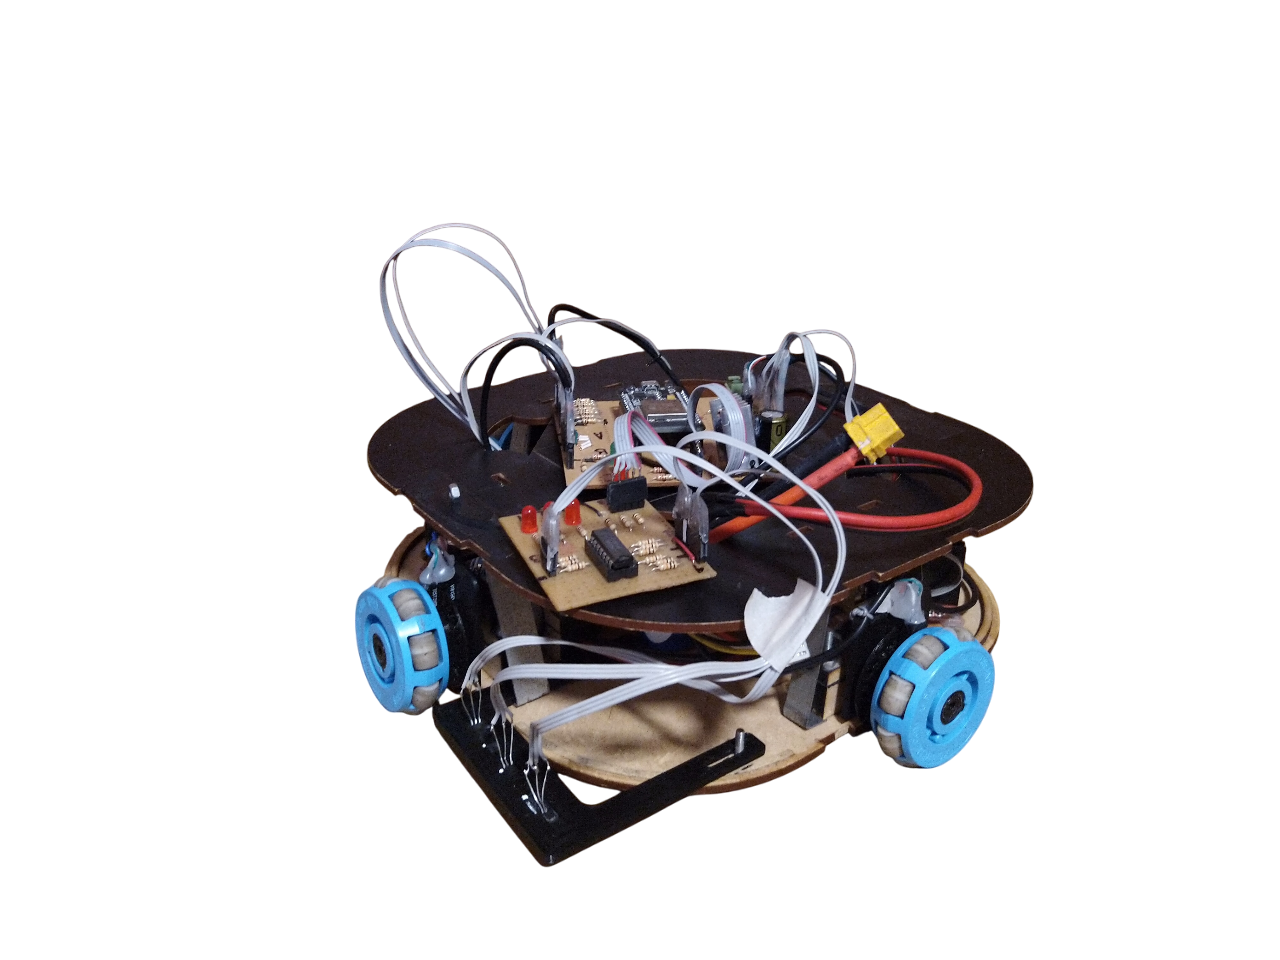
\includegraphics[trim={0 2cm 0 7.5cm}, clip, width=1.1\linewidth]{images/prototipo_robot_con_sens_mag.png}
    \caption{Prototipo del robot con seguidor de linea}
    \label{fig:prototiporobotlinef}
\end{figure}

\subsection{Riesgos superados}

Dado el desarrollo de esta iteración, se logro avanzar sobre el riesgo RI-03 y RI-01 por demostrar que los componentes elegidos aun son viables para escalar el proyecto pero existe lugar para mayor aprovechamiento de los mismos.

Por otra parte, se trabajó en superar el riesgo RI-02 por lograr una comunicación efectiva entre los componentes del sistema y se supera en parte el riesgo RI-05 al ser los nuevos componentes agregados de alta disponibilidad.

\begin{center} \begin{tabular}{|c|c|}
    \hline
        ID & Riesgo \\
    \hline
        RI-01 & Incompatibilidad o avería de componentes \\
    \hline
        RI-02 & Intercomunicación de componentes ineficiente o ineficaz \\
    \hline
        RI-03 & Prestaciones insuficientes de componentes \\
    \hline
        RI-05 & Dificultad en conseguir determinados componentes. \\
    \hline
\end{tabular} \end{center}

\subsection{Conclusiones}

Con la realización de esta iteración, obtuvimos que la implementación de compensaciones en el sistema de control marcó un hito al optimizar aspectos clave como la precisión, la estabilidad y la adaptabilidad del sistema frente a distintas condiciones de operación. Estos logros no solo demuestran la efectividad de las estrategias propuestas, sino que también refuerzan la importancia de un enfoque continuo hacia la mejora y la innovación del proyecto.
